\documentclass{article}

\usepackage{color}
\usepackage{graphicx}
\usepackage{amsmath}
\usepackage{bm}
\usepackage{enumerate}
\usepackage{booktabs}
\usepackage{cite}
\usepackage{geometry}
\usepackage{url}
\usepackage{float}
\usepackage{indentfirst}
\usepackage{ulem}
\usepackage{multirow}
\begin{document}

\vspace*{0.25cm}

\hrulefill

\thispagestyle{empty}

\begin{center}
\begin{large}
\sc{UM--SJTU Joint Institute \vspace{0.3em} \\ Introduction to Circuits \\(Ve215)}
\end{large}

\hrulefill

\vspace*{5cm}
\begin{Large}
\sc{{Laboratory Report}}
\end{Large}

\vspace{2em}

\begin{large}
\sc{{Lab 3
\vspace{0.5em}

Transient Lab}}
\end{large}
\end{center}
\vfill

\begin{table}[h!]
\centering
\begin{tabular}{ll}
Name: Kang Jiaming \hspace*{2em}&
ID: 518021911220\hspace*{2em}\\

\\

Date:  2019.10.30

\end{tabular}
\end{table}

\hfill
\newpage

\section{Introduction}

	\subsection{Objectives}

\begin{enumerate}
\item Apply the theory you learned on the step responses in first- and second-order circuits to series $RC$ and $RLC$ circuits, which you will build in the lab. 
\item Build  a series $RC$ circuit,  observe its responses  to input  square wave signal of varied frequency, and explain them based on the theory you learned.
\begin{enumerate}
\item Relate the observed capacitor voltage and resistor voltage as functions of time to your pre-lab calculations
\item Explain the changes of both output waveforms in response to the increase of the frequency of the input square wave signal
\item Explain the amplitudes of the capacitor voltage and the resistor voltage related to the amplitude of the input square wave
\end{enumerate}
\item Build a series $RLC$ circuit, observe the three types of its responses to input square wave signal, and relate them to the theory you have learned. For the under-damped/ over-damped/ critical damped response, compare the resistance in the circuit measured in the lab with the critical resistance you calculated in the pre-lab. 
\item Build the simplest second-order circuit, an $LC$ tank, and observe oscillations.
\end{enumerate}

	\subsection{Theoretical Background}
		\subsubsection{First-order circuits}

Theoretically, the transient responses in electric circuits are described by differential equations. The circuits, whose responses obey the first-order differential equation 
$$\frac{\mathrm{d}x(t)}{\mathrm{d}t} + \frac{1}{\tau}\cdot x(t) = f(t)$$
are called $\textbf{first-order circuits}$. Their  responses  are always monotonic and appear in the form of exponential function  
$$x(t) = K_1 \cdot e^{-\frac{t}{\tau}} + K_2.$$

A first-order circuit includes the effective resistance $R$ and one energy-storage element, an inductor $L$ or a capacitor $C$.

In an $RC$ circuit, the time constant is
$$\tau = RC.$$

In an $LC$ circuit, the time constant is
$$\tau = \frac{L}{R}.$$

The $\textbf{fall time}$ of a signal is defined as the interval between the moment when the signal reaches its $90\%$ and the moment when the signal reaches its $10\%$ level. Note that the $10\%$ level is reached between $2\tau$ and $3\tau$. Approximately, you can assume $falltime \approx 2.2\tau$. After $t=5\tau$, the exponent equals zero.

		\subsubsection{Second-order circuits}

Many circuits involve two energy-storing elements, both an inductor $L$ and a capacitor $C$. Such circuits require a second-order differential equation description
$$\frac{\mathrm{d}^2x(t)}{\mathrm{d}t^2} + 2\alpha\frac{\mathrm{d}x(t)}{\mathrm{d}t} + \omega_0^2x(t) = f(t),$$
and thus they are called $\textbf{second-order circuits}$.

We will  consider only second-order circuits with one inductor and one capacitor. The differential equation includes two parameters: the damping factor $\alpha$ and the undamped frequency $\omega_0$ which are determined by the circuit and its components.

For example, in the series $RLC$ circuit, which you will build and study in this lab,
$$\alpha = \frac{R}{2L}, \omega_0 = \frac{1}{\sqrt{LC}},$$
while in the parallel $RLC$ circuit,
$$\alpha = \frac{1}{2RC}, \omega_0 = \frac{1}{\sqrt{LC}}.$$

Depending on the two parameters $\alpha$ and $\omega_0$ , second-order circuits can exhibit three types of responses. 

		\subsubsection{The underdamped response}

If $\alpha < \omega_0$, 
$$x(t) = e^{\alpha t}(K_1\cos(\omega t)+K_2\sin(\omega t)),$$
where $\omega = \sqrt{\omega_0^2 - \alpha^2}$.

The underdamped circuit response involves decaying oscillations, which may last for many periods or for less than one period, depending on the damping ratio $\xi = \frac{\alpha}{\omega_0}$ , which for the series $RLC$ circuit $\xi = \frac{R}{2L} \sqrt{LC} = \frac{R}{2}\sqrt{\frac{C}{L}}$. Varying the values of $R, L, C$ affects the damping ratio $\xi$. 

		\subsubsection{The critically damped response}
If $\alpha = \omega_0$,
$$x(t) = e^{-\alpha t}(K_1 + K_2 t)$$
and the circuit has the critically damped response. The critically damped response does not involve oscillations. For the series $RLC$ circuits, $\alpha = \omega_0$ corresponds to $\frac{R}{2L} = \frac{1}{\sqrt{LC}}$ or $R_{\text{critical}} = 2\sqrt{\frac{L}{C}}$. If $L=1mH$ and $C=10nF$, then $R_{critical} \approx 632\Omega$.

		\subsubsection{The overdamped response}\
If $\alpha > \omega_0$, 
$$x(t) = K_1e^{s_1 t}+K_2e^{s_2t},$$
where $S_1 = -\alpha +\sqrt{\alpha^2-\omega_0^2}$ and $s_2 = -\alpha -\sqrt{\alpha^2 - \omega_0^2}$.

In the series $RLC$ circuits,the overdamped solution is obtained if the resistance is larger that the critical resistance, such that $R > R_{\text{critical}}=2 \sqrt{\frac{L}{C}}$. 

Notice that the larger resistance corresponds to the longer delay, and even the faster decay has a much longer fall time than the critically damped response. 

One of the most interesting features of series RLC circuits is that increasing the
resistance above the critical value results in much longer fall time, or longer delays
of responses in digital circuits. Among all monotonic responses, the critically
damped is the fastest.

\section{Results and Discussion}

	\subsection{First-order circuit}

The data for the first-order $RC$ circuit are shown in Table \ref{Table1st}.

\begin{table}[H]
\centering
\begin{tabular}{ccc}
\toprule
 & Fastest circuit response & Slowest circuit response\\
\midrule
$R_1\,\,[\text{k}\Omega]$ & 1 & 1\\
$R_p\,\,[\text{k}\Omega]$ & 0 & 10\\
$C\,\,[\mu\text{F}]$ & 0.1 & 0.1\\
Input $V_{ppk}$ [V] & 1.03 & 1.05\\
Output $V_{ppk}$ [V] & 1.04 & 1.03\\
Period of input square wave $T$ [ms] & 10 & 10\\
Output voltage rise time [ms] & 0.218 & 1.84\\
Output voltage fall time [ms] & 0.202 & 1.80\\
\bottomrule
\end{tabular}
\caption{Data for the first-order $RC$ circuit.}\label{Table1st}
\end{table}

In theory, we can calculate that for the fastest circuit response, the time constant $\tau_1$ and the fall time are
$$\tau_1 = (R_1+R_p)C = 1000 \times 0.1 \times 10^{-6} = 10^{-4}\,\,[\text{s}] = 0.1\,\,[\text{ms}],$$
$$fall\,\,time = 2.2\tau_1 = 2.2 \times 0.1 = 0.22\,\,[\text{ms}].$$

The relative error is
$$\epsilon_{\text{rise time}} = \frac{0.218-0.22}{0.22}\times 100\% = 0.91\%,$$
$$\epsilon_{\text{fall time}} = \frac{0.202-0.22}{0.22}\times 100\% = 8.18\%.$$

For the slowest circuit response, the time constant $\tau_2$ and the fall time are
$$\tau_2 = (R_1+R_p)C = (10000+1000) \times 0.1 \times 10^{-6} = 1 \times 10^{-4}\,\,[\text{s}] = 1.1\,\,[\text{ms}],$$
$$fall\,\,time= 2.2\tau_2 = 2.2 \times 1.1 = 2.42\,\,[\text{ms}].$$

The relative error is
$$\epsilon_{\text{rise time}} = \frac{2.352-2.42}{2.42}\times 100\% = -23.9\%,$$
$$\epsilon_{\text{fall time}} = \frac{2.252-2.42}{2.42} \times 100\% = -25.6\%.$$

The relative error for the measurement results of the rise time and fall time of the slowest circuit response is unsatisfying. Such big deviation from the theoretical value may originate from our wrong operation of the oscillator.

	\subsection{Second-order circuit}

In the $RLC$ series circuit in this lab, $L = 1$ mH, $R_2 = 100\,\,\Omega$, $C = 820$ pF,
$$R_{{\text{critical}}} = 2\sqrt{\frac{L}{C}} - R_2 = 2.109\,\,[\text{k}\Omega]$$
The data for the $RLC$ series circuit are shown in Table \ref{Table2nd}

\begin{table}[H]
\centering
\begin{tabular}{ccccc}
\toprule
& $R_p\,\,[\text{k}\Omega]$ & Rise time [ms] & Fall time [ms] & time interval $\Delta t$ [$\mu$s]\\
\hline
\multirow{2}{*}{Under-damped} & 0 & 0.062 & 0.047 & 3.20 \\
& 1 & 1.75 $\times 10^{-3}$ & 1.89 $\times 10^{-3}$ & 50.0 \\
\hline
Critically damped  & 2 & 3.75 $\times 10^{-3}$ & 3.72 $\times 10^{-3}$ & 49.8\\
\multirow{2}{*}{Over-damped} & 3 & 6.07$\times 10^{-3}$ & 5.85 $\times 10^{-3}$ & 49.8\\
& 4 & 8.59 $\times 10^{-3}$ & 7.94 $\times 10^{-3}$ & 49.8\\
\hline
\end{tabular}
\caption{Data for the second-order $RLC$ series circuit.}\label{Table2nd}
\end{table}

The oscillograms for each case are presented below (Figure \ref{FigU1} $\sim$ \ref{FigO2}).

\begin{figure}[H]
\centering
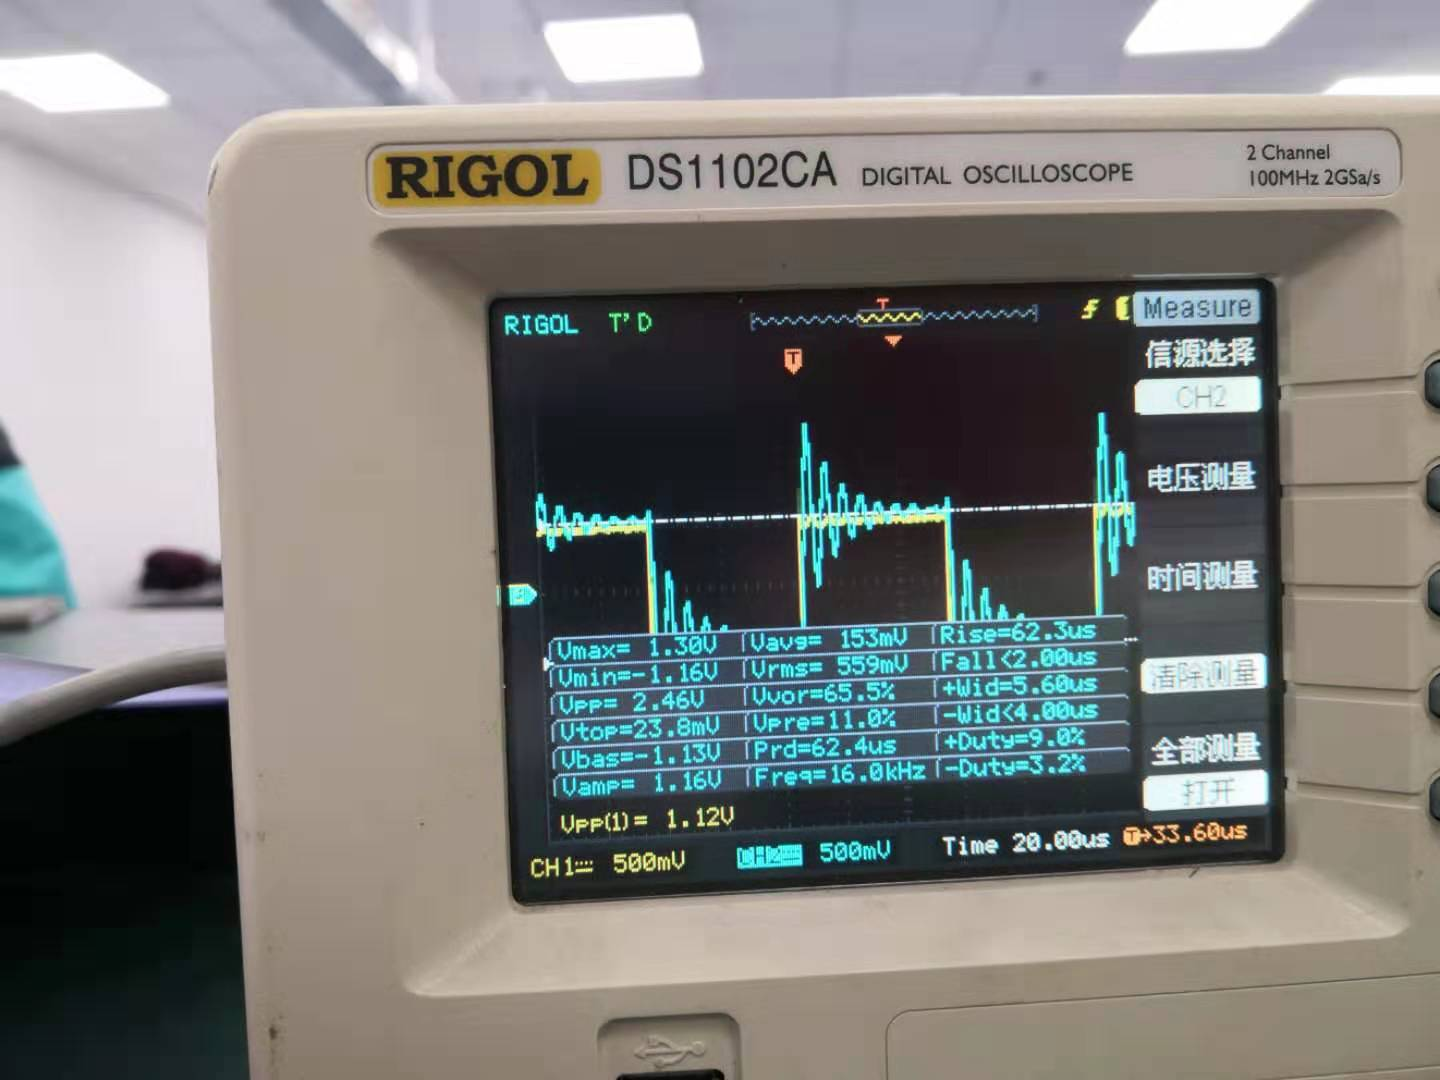
\includegraphics[scale=0.25]{1.jpg}
\caption{Oscillogram for $R_p=47.3\times 10^{-3}\text{k}\Omega$ (underdamped).}\label{FigU1}
\end{figure}

\begin{figure}[H]
\centering
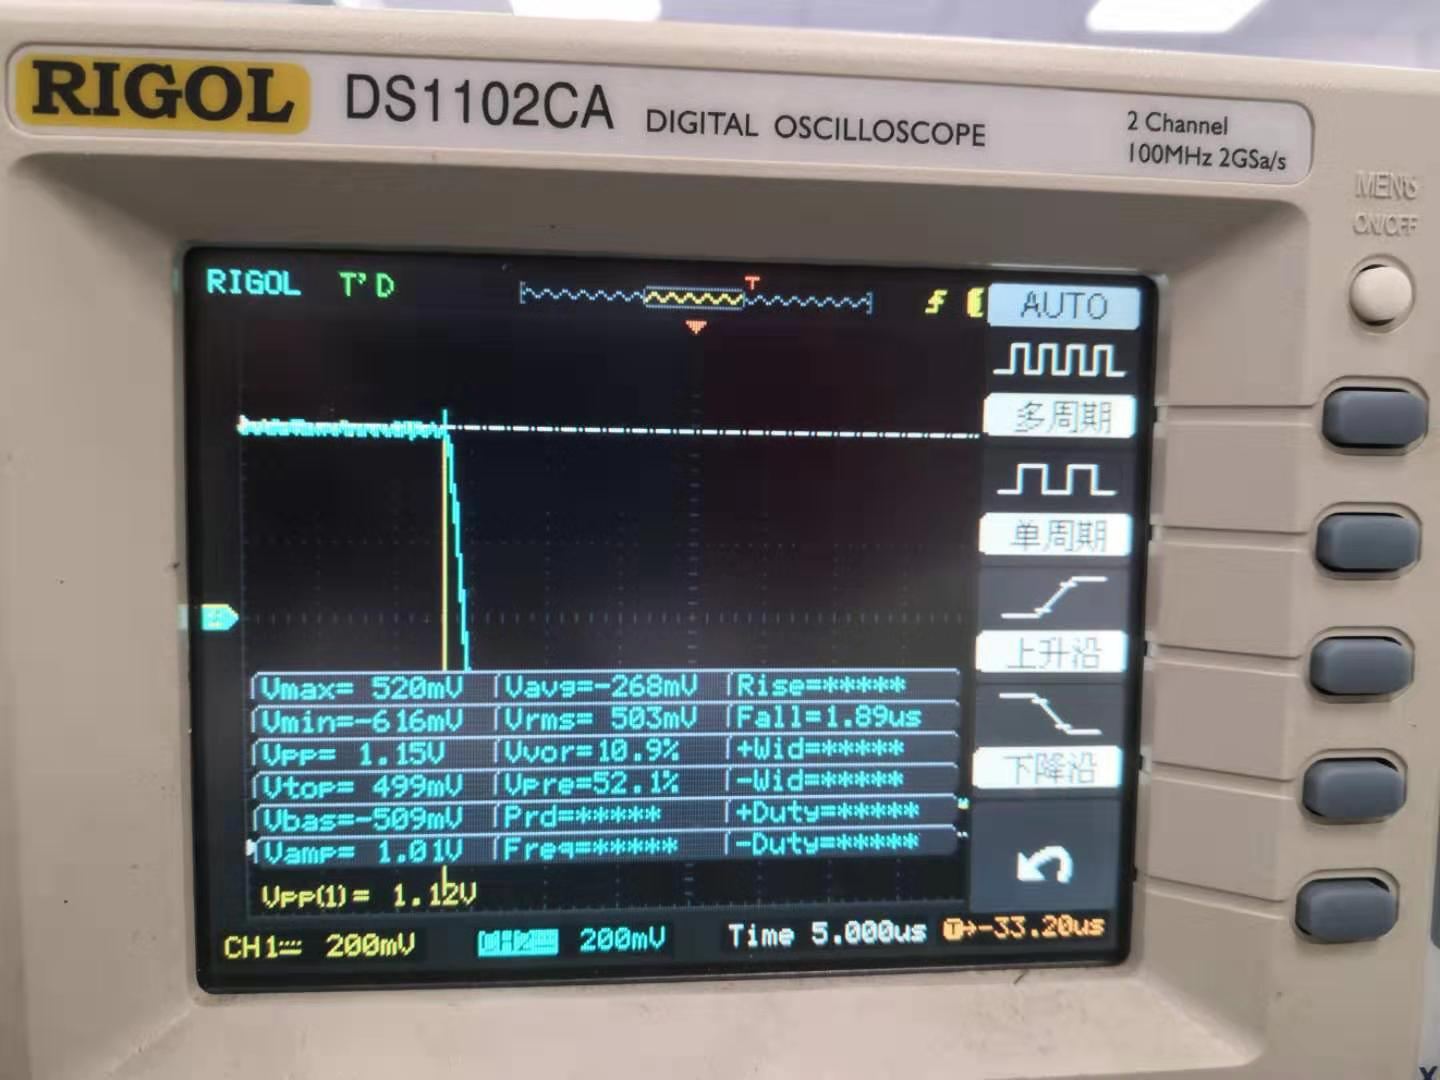
\includegraphics[scale=0.15]{3.jpg}
\caption{Oscillogram for $R_p=1.09\,\,\text{k}\Omega$ (underdamped).} \label{FigU2}                                                        \end{figure}

\begin{figure}[H]
\centering
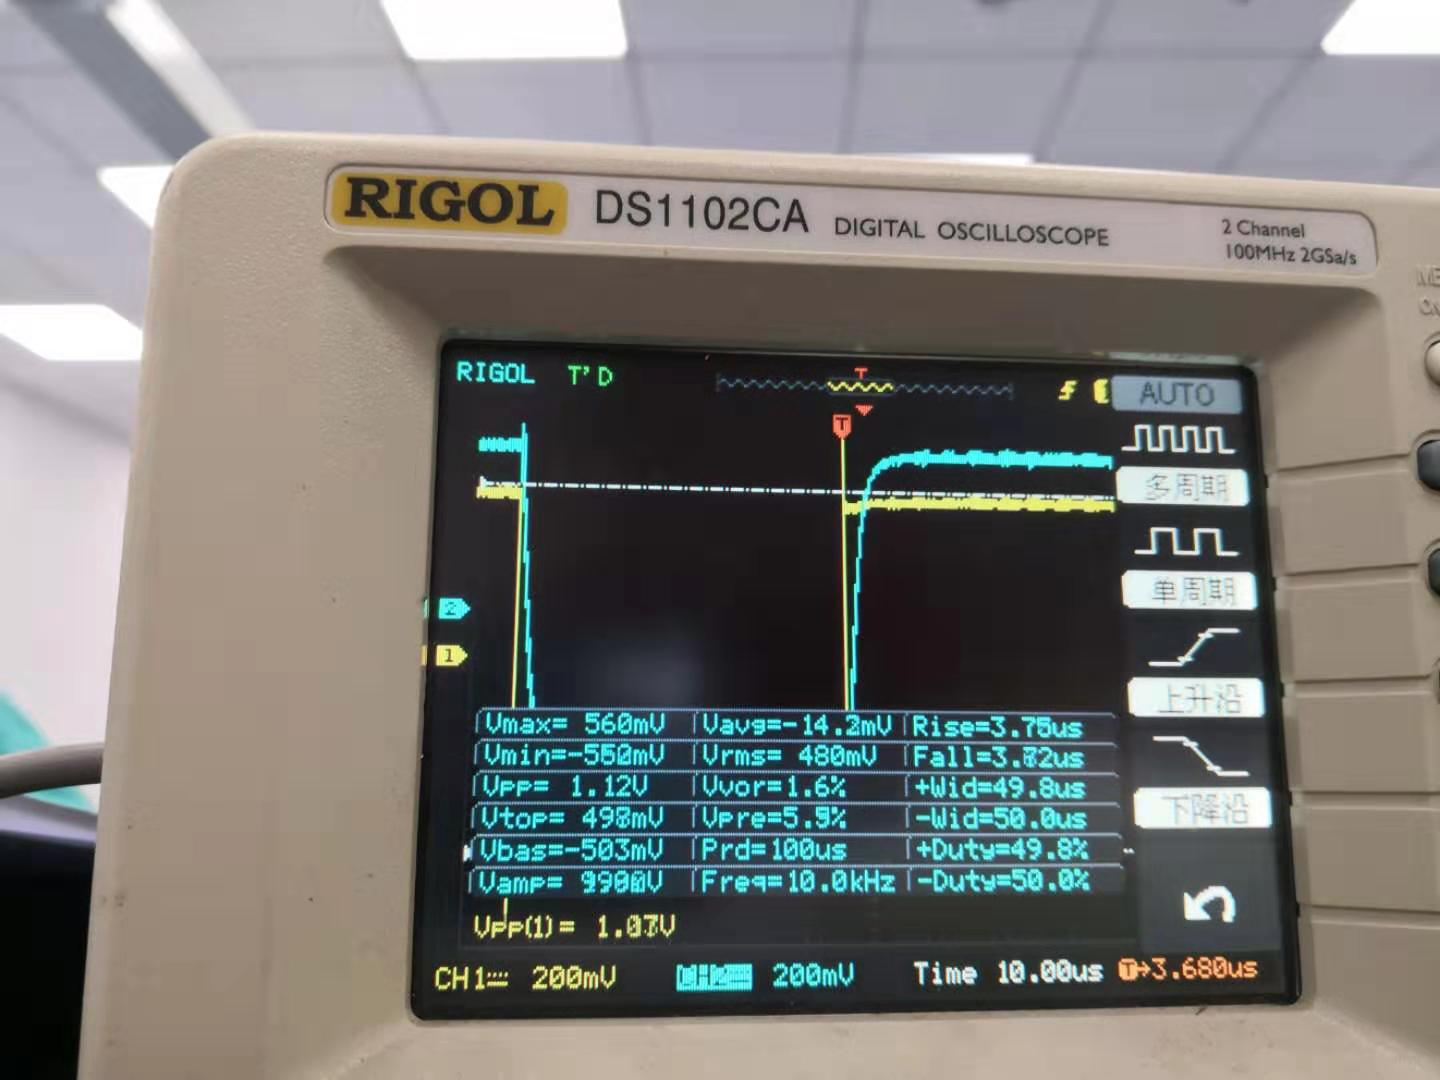
\includegraphics[scale=0.27]{4.jpg}
\caption{Oscillogram for $R_p=2.07\,\,\text{k}\Omega$ (critically damped).}\label{FigC}
\end{figure}

\begin{figure}[H]
\centering
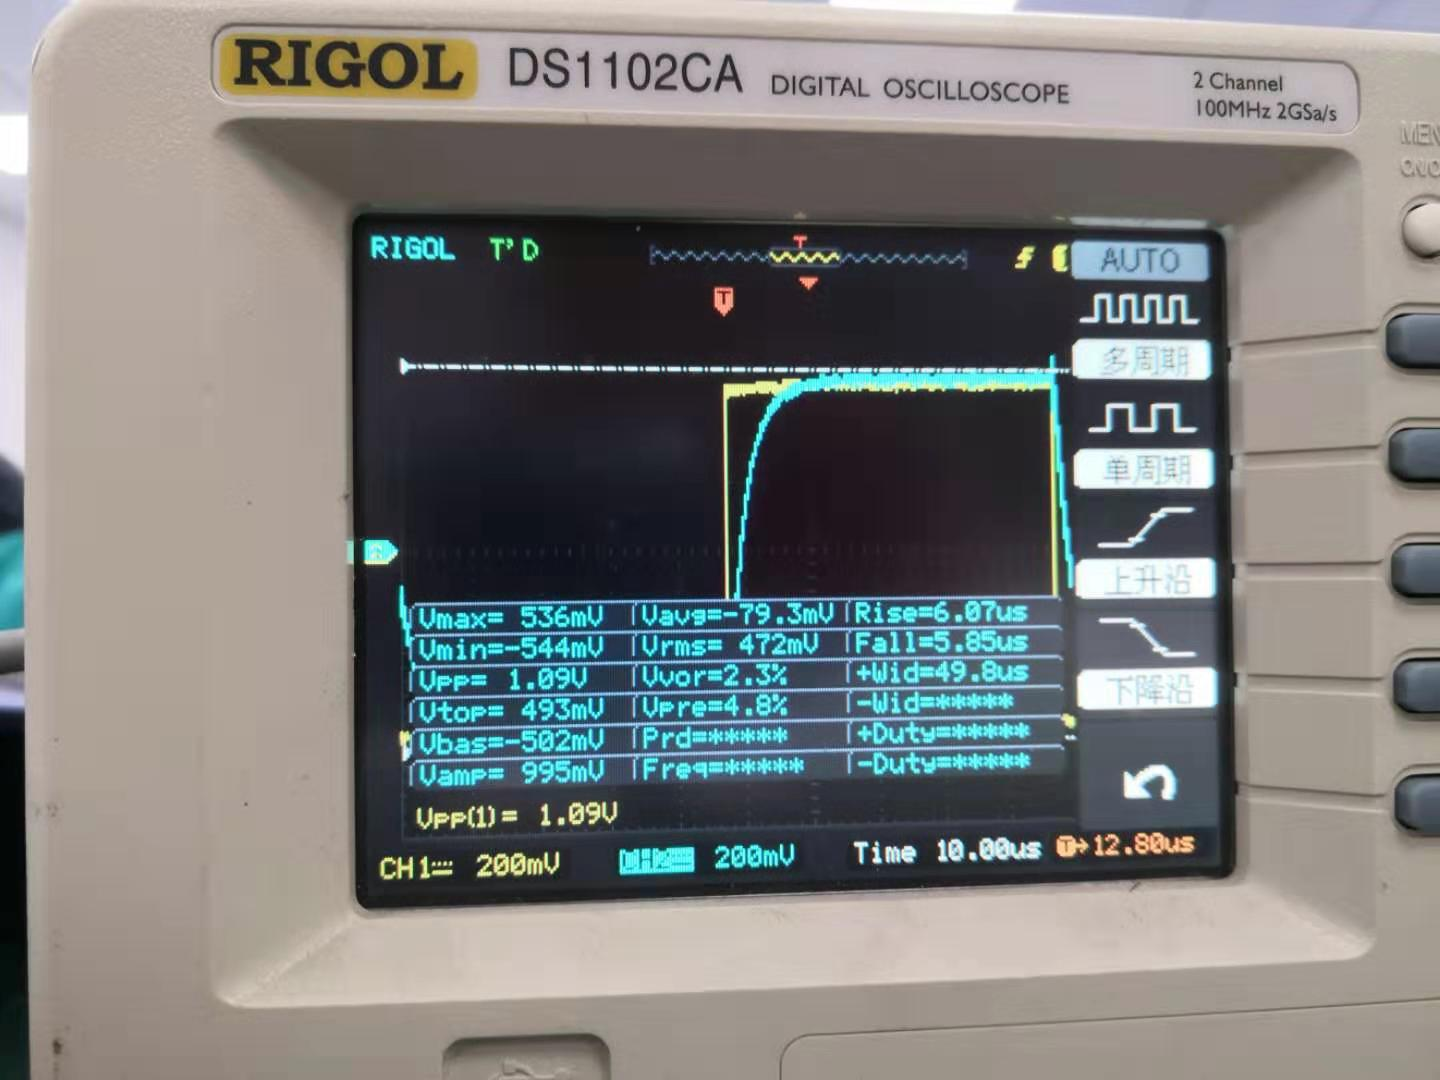
\includegraphics[scale=0.22]{5.jpg}
\caption{Oscillogram for $R_p=3.10\,\,\text{k}\Omega$ (overdamped).}\label{FigO1}
\end{figure}

\begin{figure}[H]
\centering
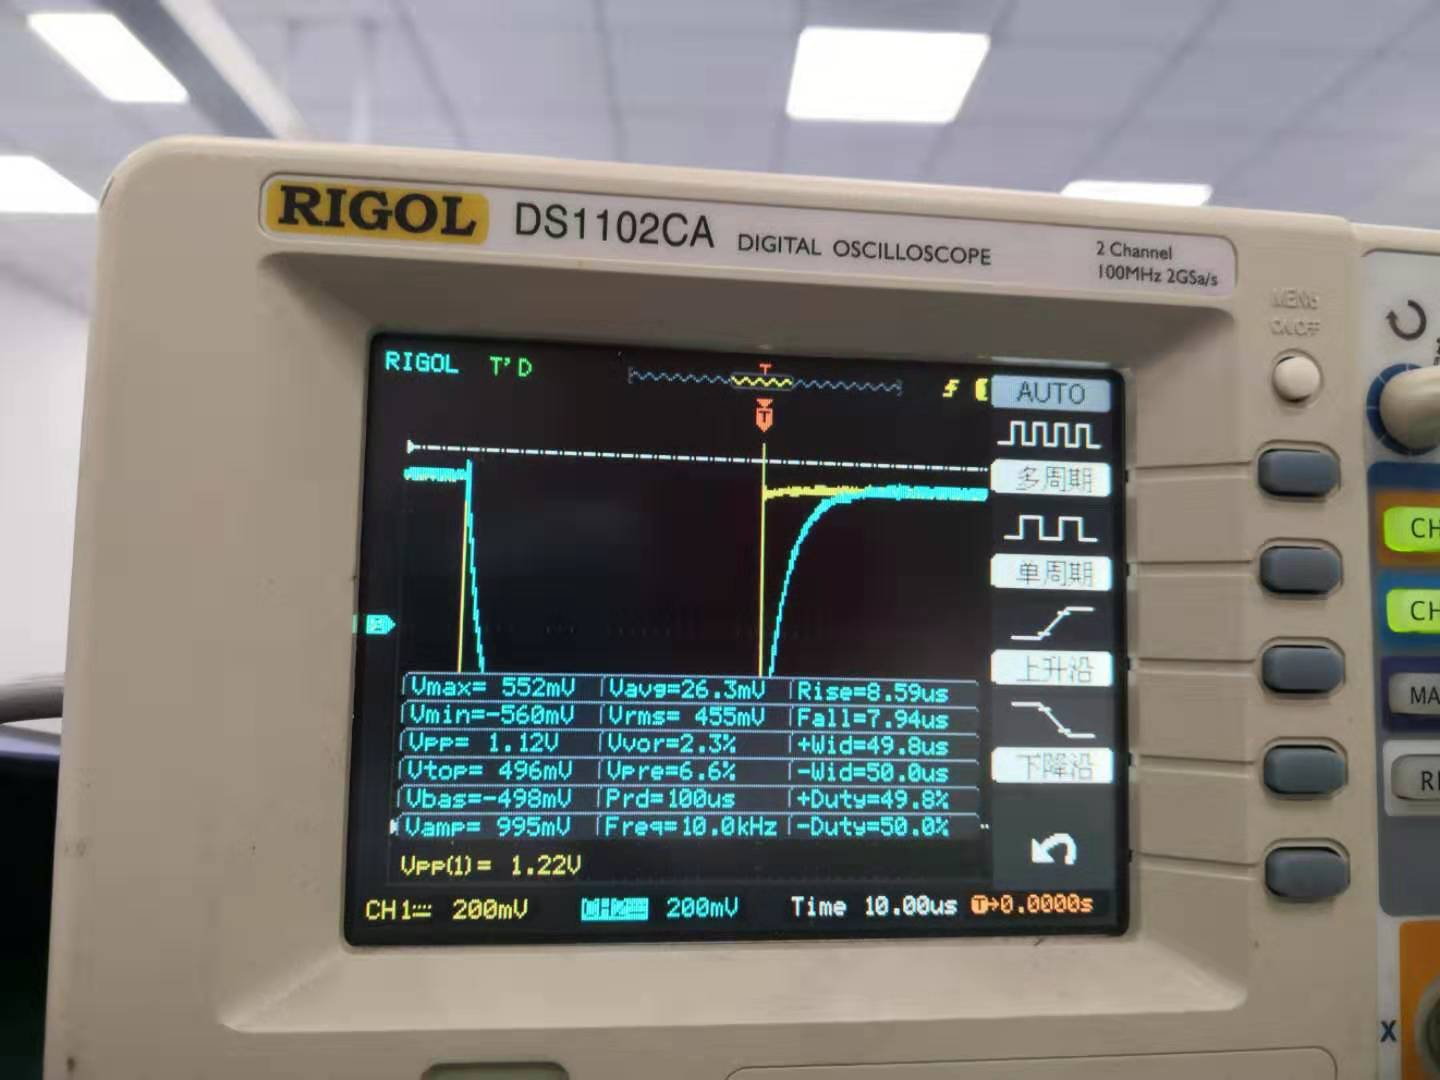
\includegraphics[scale=0.22]{6.jpg}
\caption{Oscillogram for $R_p=5.96\,\,\text{k}\Omega$ (overdamped).}\label{FigO2}
\end{figure}

Actually, only the oscillogram for the first wave is properly recorded. This is because for the other cases, when the waveform is properly displayed, the fall time cannot be measured and we had to adjust the scale. Though the oscillograms are not recorded, we had checked that the output waveforms all conformed to the theoretical shapes.

There is an obvious mistake in our measurement of the time interval, since the time interval for the last three cases should not exist since the output voltage is always positive. This mistake may occur due to our wrong operation of the device.

\section{Conclusions}

In the lab 3, we got familiar with the $RC$ circuit and $RLC$ circuit. We also got to know some new concepts of circuit, such as the fall time and the rise time. We explored constructing these two type of circuits and we examined the response of first-order $RC$ circuit and the three types of responses of the second-order $RLC$ series circuit.

Though some of our experimental results are accompanied with a relatively large error and some oscillograms are not recorded properly, the main points of this experiment are verified in our experiment.

One of the most confusing points of this lab is how to operate the oscillator properly and efficiently. If we can get lectured on that, I believe that the experiment can be carried out more correctly and effectively.

\section{References}

\noindent [1] VE215 \hspace{0.5em} Lab3: Transient Lab lab manual.

\section{Appendix}

Please find the original data sheet at the end of the report.


\end{document}